\documentclass[10pt,twocolumn]{scrartcl}

\usepackage[utf8]{inputenc}
\usepackage[T1]{fontenc}
\usepackage[ngerman]{babel}

\usepackage{lmodern}
\usepackage[sc]{mathpazo} % or option osf
\usepackage{newpxmath}
\usepackage[scaled = 0.85]{beramono}

\usepackage{xpatch}
\usepackage{xcolor}
\usepackage{realboxes}
\definecolor{mygray}{rgb}{0.9,0.9,0.9}
\usepackage{listings}
\lstdefinelanguage{commentonly}{ morecomment=[l]{\#} }
\lstset{literate=%
{Ö}{{\"O}}1
{Ä}{{\"A}}1
{Ü}{{\"U}}1
{ß}{{\ss}}2
{ü}{{\"u}}1
{ä}{{\"a}}1
{ö}{{\"o}}1
,basicstyle=\ttfamily
,backgroundcolor=\color{mygray}
,commentstyle=\emph
,language=commentonly
,upquote=true
}
\makeatletter
\xpretocmd\lstinline{\Colorbox{mygray}\bgroup\appto\lst@DeInit{\egroup}}{}{}
\makeatother

\usepackage{enumitem}

\usepackage{adjustbox}
\usepackage[a4paper, margin=1mm, includefoot, footskip=15pt]{geometry}

\usepackage[pdftitle={Eine kurze Einführung in die Sprache Julia}
, pdfauthor={Georg Kindermann}
, pdfsubject={Julia}
, pdfkeywords={Julia, Lang, Progammiersprache, Tutorial, German, Deutsch}
, pdflang={de-AT-1996}
, colorlinks=true
, linkcolor=blue
, urlcolor=blue
, pdfpagemode=UseNone]{hyperref}

\nonfrenchspacing
\sloppy

\title{Eine kurze Einführung in die Sprache Julia}
\author{Georg Kindermann}
%\date{19. Juni 2023}

\begin{document}

\maketitle

%\begin{abstract}
%  Eine kurze Einführung in die Sprache Julia.
%\end{abstract}

\tableofcontents

\section{Einleitung}
\label{sec:einleitung}

\href{https://julialang.org/}{Julia} kann mit
\href{https://github.com/JuliaLang/juliaup}{juliaup} installiert werden. Dies
ist keine \href{https://docs.julialang.org/en/v1/}{ausführliche Anleitung},
sondern lediglich ein kurzer Überblick und orientiert sich am
\href{https://github.com/bkamins/The-Julia-Express}{Julia Express} von Bogumił Kamiński.

Mithilfe der REPL (read-eval-print loop) kann Julia interaktiv benutzt werden.
Als IDE (integrierte Entwicklungsumgebung) wird
\href{https://www.julia-vscode.org/}{VS code mit dem Julia plugin} empfohlen. Die gezeigten Codeabschnitte wurden mit Version 1.9.1 (2023-06-07) getestet.

\section{REPL}
\label{sec:repl}

Wenn man \lstinline|julia| startet, kommt man in den interaktiven Modus (REPL).
Deren wichtigsten Kommandos sind:
\begin{description}[style=multiline,leftmargin=2cm,nolistsep]
  \item[CTRL+d] Beendet Julia
  \item[CTRL+c] Bricht Berechnungen ab
  \item[?] Hilfe--Modus
  \item[;] Shell--Modus
  \item[{]}] Packetmanager--Modus
  \item[{]?}] Hilfe zum Packetmanager
  \item[Backspace] Modus verlassen
  \item[CTRL+l] Bildschirm löschen
\end{description}
In der REPL wird nach jedem Befehl dessen Wert ausgegeben. Wenn man
\lstinline|;| am Ende des Befehls setzt, wird der Wert nicht ausgegeben. Mit
\lstinline|?cos| bekommt man die Hilfe zu \lstinline|cos|. Mit
\lstinline|]add [package name]| wird das Paket
\lstinline|[package name]| installiert und mit
\lstinline|]up| werden alle bereits installierten Pakete aktualisiert.

Ein paar wichtige Funktionen sind:

\begin{lstlisting}
versioninfo()       # Zeigt Version
varinfo()           # Zeigt globale Variablen
pwd()               # Aktuelles Verzeichnis
cd("D:/")           # Wechsle Verzeichnis
include("file.jl")  # Führt Datei aus
exit()              # Beendet Julia
@edit sin(1)        # Zeigt definition von sin
\end{lstlisting}

Skripts können mit \lstinline|julia script.jl| ausgeführt werden.

\section{Grundtypen}
\label{sec:grundtypen}

Mit \lstinline|x::Type| wird \lstinline|x| mit dem Typ \lstinline|Type| erzeugt.
Integer sind auf 32~Bit Systemen 32~Bit und auf 64~Bit Systemen 64~Bit.
\lstinline|1::Int32| geht nur auf 32 \lstinline|1::Int64| auf 64~Bit Systemen. 

\begin{lstlisting}
1             # Integer
1::Int        # Integer Explizit
1.0           # Float
1.0::Float64  # Float Explizit
true::Bool    # Boolean false
'c'::Char     # Character 1 Zeichen
"s"::String   # String n Zeichen
\end{lstlisting}

Mit \lstinline|T(x)| wird ein Wert \lstinline|x| vom Typ \lstinline|T| erzeugt.

\begin{lstlisting}
Int32(1)           # 32 Bit Integer
Int64(1)           # 64 Bit Integer
Int64(2.0)         # Float als Integer
#Int64(1.3)        ## InexactError
floor(Int64, 1.3)  # Abrunden
ceil(Int64, 1.3)   # Aufrunden
round(Int64, 1.3)  # Runden
\end{lstlisting}

Es gibt
\lstinline|Char|,
\lstinline|string| (kleingeschrieben),
\lstinline|Bool|,
\lstinline|Int|,
 \lstinline|Int8|,
\lstinline|Int16|,
\lstinline|Int32|,
\lstinline|Int64|,
\lstinline|Int128|,
\lstinline|UInt|,
\lstinline|UInt8|,
\lstinline|UInt16|,
\lstinline|UInt32|,
\lstinline|UInt64|,
\lstinline|UInt128|,
\lstinline|Float|,
\lstinline|Float16|,
\lstinline|Float32| und
\lstinline|Float64|.

\lstinline|string(1, true)| ergibt \lstinline|1true|. Es werden mehrere
Argumente zu einem String zusammengehängt. Einzelnen Zeichen, nicht aber
Zeichenketten, können mit \lstinline|Int64('a')| in einen Integerwert
umgewandelt werden. Mit \lstinline|Char(89)| kann ein Integerwert in ein Zeichen
umgewandelt werden. \lstinline|Bool(0)| ergibt \lstinline|false| und
\lstinline|Bool(1)| \lstinline|true|. Andere Zahlen können nicht nach Bool
umgewandelt werden. Zusätzlich kann auch mit \lstinline|convert(Int64, 1.0)|
oder \lstinline|parse(Int64, "1")| umgewandelt bzw.\ erzeugt werden.

Zusätzlich gibt es noch:
\begin{lstlisting}
123 // 456    # Rationale Zahl
1 + 1im       # Komplexe Zahl
big"1"        # BigInt
BigInt(1)     # BigInt
big"1.5"      # BigFloat
BigFloat(10)  # BigFloat
\end{lstlisting}

Die Genauigkeit von \lstinline|BigFloat| kann mit \lstinline|setprecision| eingestellt werden.

Mit \lstinline|zero(10.0)| wird eine $0$ vom gleichen Typ wie $10.0$ erzeugt.
Mit \lstinline|one(Int64)| wird eine $1$ vom Typ Int64 erzeugt.
\lstinline|promote(true, 1 // 3, 2, 1.0)| erzeugt, solange eine Konvertierung
möglich ist, einen Tuple vom gleichen Typ - hier von Float. Einige Operatoren
(Arithmetisch, Zuweisung) machen eine automatische Typumwandlung. So wird bei
\lstinline|1 + 1.0| die Integer $1$ in Float umgewandelt. Hingegen wird Bool z.\,B.\ in \lstinline|true + true| direkt als Integer verwendet. 

Den Typ kann man feststellen mit:
\begin{lstlisting}
typeof("abc")      # String
isa(1.0, Float64)  # true
1.0 isa Number     # Alternative Syntax
supertype(Int64)   # supertype von Int64
subtypes(Real)     # subtypes von Real
Int <: Real        # Ist Int subtyp von Real
\end{lstlisting}

\section{Weitere Typen}
\label{sec:weitereTypen}

\begin{lstlisting}
Any                      # Typ: Alle Objekte
Nothing                  # Typ: Nichts
nothing                  # Nichts
Missing                  # Typ: Fehlender Wert
missing                  # Fehlender Wert
ismissing(missing)       # true
coalesce(missing, 1, 2)  # Erster nicht missing Wert
\end{lstlisting}

\lstinline|undef| kann zur Erzeugung eines Arrays verwendet werden, dessen Werte
nicht initialisiert sind z\,B.\ \lstinline|Array{Float64, 1}(undef, 3)|.

\subsection{Tuple und NamedTuple}
\label{ssec:tuple}

In einem \emph{Tuple} werden unveränderbare, statische Werte von unterschiedlichen Typen abgelegt. Der Index des ersten Elements ist 1.

\begin{lstlisting}
()              # Leerer tuple
(1,)            # Tuple mit einem Element
("a", 1)        # Tuple mit zwei Element
('a', false)::Tuple{Char, Bool}  # Mit Typ
x = (1, 2, 3)
x[1]            # 1 (element)
x[1:2]          # (1, 2) (tuple)
x[[1, 3]]       # (1, 3) (tuple)
x[begin]        # Erster Wert in x
x[end]          # Letzter Wert in x
lastindex(x)    # Letzter Index von x
x[begin:2:end]  # Jedes zweite Element
#x[4]           ## BoundsError
#x[1] = 1       ## error - tuple ist statisch
a, b = x        # unpacking a=1, b=2
\end{lstlisting}

Tuple Elemente können einen Namen haben (\lstinline|NamedTuple|) und sind
vergleichbar mit einer \hyperref[ssec:composite]{anonymen \lstinline|struct|}.

\begin{lstlisting}
NamedTuple()  # Empty named Tuple
(x="a", y=1)  # Named Tuple mit 2 Elementen
x = (p=1, q=2, r=3)
x.p           # Element p von Tuple x
(; a, b, c)   # Named Tuple mit a,b,c und deren Werten
\end{lstlisting}

\subsection{Array}
\label{ssec:array}

Werte eines Arrays sind veränderbar und vom selben Typ, wobei es auch den Typ
Any gibt. Die erste Dimension ist Vertikal, die zweite Horizontal. Mit folgenden
Befehlen kann ein Array mit Werten erzeugt werden.

\begin{lstlisting}
[1]            # Vektor mit einem Element
[1;]           # Vektor mit einem Element
[1;;]          # 1x1 Matrix
[1;;;]         # 1x1x1 Array
[(1, 2)]       # Vektor mit einem Element
[1, 2]         # Vertikaler Vektor (concatenation)
[1; 2]         # Vertikaler Vektor (vcat Funktion)
[1;
 2]            # Vertikaler Vektor (vcat Funktion)
[1
 2]            # Vertikaler Vektor (vcat Funktion)
[[1,2], 3]     # 2-element Vector{Any}
[[1;2], 3]     # 2-element Vector{Any}
[[1,2]; 3]     # 3-element Vector{Int64}
[[1;2]; 3]     # 3-element Vector{Int64}
[[1,2]
 3]            # 3-element Vector{Int64}
[[1 2] 3]      # 1x3 Matrix (hcat)
[1, 2]'        # Horizontaler "Vektor" adjoint 1x2
[1 2]          # 1x2 Matrix (hcat Funktion)
[1 2]::Array{Int64, 2}  # Int64 2D Array
[1 2]::Matrix{Int64}    # Das gleiche
[1;;2]         # 1x2 Matrix
[1;;
 2]            # 1x2 Matrix
[1 2]'         # 2x1 Adjoint Matrix (gleicher Speicher)
[1, 2]' == [1 2]    # true Dimension 1x2 gleich 1x2
[1, 2] == [1 2]'    # false Dimension 2 nicht gleich 2x1
permutedims([1 2])  # 2x1 Matrix (neuer Speicher)
[1 3 5; 2 4 6]         # 2x3 Matrix (hvcat Function)
[1 3 5
 2 4 6]                # 2x3 Matrix
[1 2 4;;
 5 7 8]                # 1x6 Matrix
#[1 2 4;;5 7 8]        ## Error mix Space und ;;
[[1,2]  [3,4]  [5,6]]  # 2x3 Matrix
[[1 2]; [4 5]; [7 8]]  # 3x2 Matrix
[[1 2]  [4 5]  [7 8]]  # 1x6 Matrix
[1 3 5
 2 4 6;;;
 7 9 11
 8 10 12]              # 2x3x2 Array
\end{lstlisting}

Mit \lstinline|,| werden Elemente, so wie sie sind, zu einem Vektor aneinander
gehängt. Mit \lstinline| | (Space) und neuen Zeilen wird eine Matrix wie sie ist
erzeugt. Mit \lstinline|;| werden Elemente zu einem gemeinsamen Vektor
zusammengefügt, wobei \lstinline|;| entlang der \emph{ersten} Dimension
(Vertikal), \lstinline|;;| entlang der \emph{zweiten} Dimension (Horizontal),
\lstinline|;;;| entlang der \emph{dritten} Dimension (hintereinander), \dots
zusammenfügt.

Mit folgenden Befehlen kann ein Array uninitialisiert bzw.\ mit regelhaften
Werten erzeugt werden.

\begin{lstlisting}
Array{Int}(undef, 2)        # 2-element Vector{Int64}
Vector{Int}(undef, 2)       # 2-element Vector{Int64}
Array{Int}(undef, 2, 3)     # 2x3 Matrix{Int64}:
Matrix{Int}(undef, 2, 3)    # 2x3 Matrix{Int64}:
Array{Int}(undef, 2, 3, 4)  # 2x3x4 Array{Int64, 3}
falses(3)            # Vektor mit 3 true
trues(3)             # Vektor mit 3 false
zeros(3)             # Vektor mit 3 Float64 Nuller
ones(3)              # Vektor mit 3 Float64 Einser
ones(Int64, 2, 3)    # 2x3 Matrix Int64 Einser
x = range(0, 1, 11)  # Iterator 0 bis 1 mit 11 Elementen
collect(x)           # Wandelt Iterator in Vector um
1:10                 # Iterator 1 bis 10
1:2:10               # Iterator 1 bis 10 in 2er Schritten
reshape(1:12, 3, 4)  # 3x4 "Matrix" spaltenweise gefüllt
fill(7, 2, 3)        # 2x3 Matrix gefüllt mit 7
repeat([[1,2] [3,4]], 2, 3) # 2x2 Matrix 2x3 mal -> 4x6
stack([[1,2], [3,4]])  # Mehrere Arrays kombinieren
stack([[1,2], [3,4]], dims=1) # Horizontal
x = [1, 2]       # 2-element Vector
resize!(x, 5)    # Hängt 3 uninitialisiert Elemente an
collect((1, 2))  # unpacking Vektor aus Tuple
tuple([1,2,3])   # 1-Element Tuple mit dem Vektor
Tuple([1,2,3])   # unpacking Tuple aus Vektor
\end{lstlisting}

Mit \emph{Comprehensions} können Arrays mithilfe von Schleifen und Funktionen erzeugt werden.

\begin{lstlisting}
[x * y for x in 1:2, y in 1:3]    # 2x3 Array
[x * y for x in 1:2 for y in 1:3] # 6-element Vektor
Float64[x^2 for x in -2:2]        # Typecast nach Float64
[x * y for x in 1:2, y in 1, z in 1:3]   # 2x3 Array
[x * y for x in 1:2, y in 1:1, z in 1:3] # 2x1x3 Array
[x * y for x=1:3 for y=1:x if x+y == 4]  # Mit Bedingung
\end{lstlisting}

Eine Dimension mit nur einem Element wird automatisch entfernt. Falls sie
erhalten bleiben soll, muss z.\,B.\ statt \lstinline|1| \lstinline|1:1|
geschrieben werden.

Weitere wichtige Funktionen im Umgang mit Arrays sind:
\begin{lstlisting}
A = rand(2,1,3)      # 2x1x3 Array{Int64, 3}
ndims(A)             # Anzahl Dimensionen: 3
eltype(A)            # Type der Elemente: Float64
length(A)            # Anzahl Elemente: 6
size(A)              # Tuple mit Dim. Längen: (2, 1, 3)
axes(A)              # Tuple mit Ranges der Dimensionen
 # (Base.OneTo(2), Base.OneTo(1), Base.OneTo(3))
eachindex(A)     # Eindimesnionaler Index: Base.OneTo(6)
CartesianIndices(A)  # Lazy Index Iterator von A
 # CartesianIndices((2, 1, 3))
LinearIndices(A)     # Lazy linear Iterator von A
 # 2x1x3 LinearIndices{3, Tuple{Base.OneTo{Int64},
 #  Base.OneTo{Int64}, Base.OneTo{Int64}}}:
vec(A)               # Array als Vector reuse memory
 # 6-element Vector{Float64}
dropdims(A, dims=2)  # Zweite Dim. ist 1 lang
 # 2x3 Matrix{Float64}
sum(A, dims=3)       # Summe über die 3 Dimension
 # 2x1x1 Array{Float64, 3}:
sum(A, dims=(1,2))   # 1x1x3 Array{Float64, 3}
sum(A, dims=[1,2])   # 1x1x3 Array{Float64, 3}
count(>(0.5), A)     # Anzahl Werte in A > 0.5
 # Mit der anonymen Funktion >(0.5)
any(>(0.5), A)       # Irengt ein Wert > 0.5: true/false
all(>(0.5), A)       # Alle Werte > 0.5: true/false
\end{lstlisting}

Auf Array--Elemente kann genauso zugegriffen werden wie auf
\hyperref[ssec:tuple]{Tuple--Elemente}. Auch wenn mehrere Dimensionen bestehen,
gibt es die Möglichkeit auf die einzelnen Elemente linear zuzugreifen, so als ob
es sich um einen Vektor handeln würde. Zusätzlich gibt es noch folgende
Zugriffsmöglichkeiten:

\begin{lstlisting}
A = reshape(collect(1:24), (2, 3, :))  # 2x3x4 Array
A[[true, false], [3, 1], 1]            # 1x2 Matrix
A[1, :, 1:2]          # : für alles: 3x2 Matrix
A[1:1, 1, :]          # 1x4 Matrix
A[1, 1, :]            # 4-element Vector
A[1, 1, :, [true]]    # 4x1 Matrix
A[1, 1, :, [false]]   # 4x0 Matrix
A[[1, 7, 3]]          # Als Vektorindex: 3-element Vector
A[[1 7 3]]            # Gleiche Daten aber: 1x3 Matrix
A[[1 7 3; 2 5 7]]     # 2x3 Matrix
A[2, [1 2; 3 1], 4]   # 2x2 Matrix
A[1, 1, 2:3]          # 2-element Vector
A[1, 1, 2:end-1]      # Hier das Gleiche wie zuvor
view(A, [1, 9])  # SubVektor von A, Zeigt auf Daten von A
view(A, 1:2, 2:3, 4)  # Subarray-View
\end{lstlisting}

Daten eines Arrays verändern.

\begin{lstlisting}
A = reshape(Vector(1:12), (3, 4))  # 3x4 Matrix
A[2, 1] = 3         # Element 2, 1 wird auf 3 gesetzt
#A[:, 2:3] = 3      ## Error size mismatch
A[:, 2:3] .= 3      # OK, broadcasting mit .
A[:, 2:3] .= [1 2]  # Atomatisch wiederholt
A[:, 2:3] = repeat([1 2], 3)  # das gleiche
x = A[:, 2:3]       # Macht ein neues Array x
x .= 4              # Werte in x aber nicht in A geändert
y = view(A, :, 2:3) # Zeigt auf Daten in A
y .= 5              # Werte in A geändert
\end{lstlisting}

Ein Array wird als \emph{Referenz} übergeben, d.\,h.\ wenn Werte verändert
werden, ist dies in allen Referenzen zu sehen. Mit \lstinline|copy| kann die
äußere Struktur, mit \lstinline|deepcopy| alle Daten rekursiv kopiert werden. 

\begin{lstlisting}
A = [[2, 1], 1]  # 2-element Vector{Any}
x = A            # Refernz auf A
y = copy(A)      # Struktur von A
z = deepcopy(A)  # Rekrusive Kopie von A
A[1][1] = 0      # Inplace Veränderung
A[2] = 3.        # Neues Element
x                # Indentisch mit neuem A
y                # Nur Veränderung von A[1][1]
z                # Inhalt wie ursprüngliches A
\end{lstlisting}

Zahlen werden wie Vektoren mit genau einem Element verarbeitet.
\begin{lstlisting}
x = 10
x[]       # 10
x[1]      # 10
x[1, 1]   # 10, alle 1 am Ende werden ignoriert
only(x)   # 10
size(x)   # (), Leerer Tuple
y = [10]  # 1-element Vector
y[]       # 10, Geht nur bei Arrays mit genau 1 element
only(y)   # 10, Geht nur bei Arrays mit genau 1 element
size(y)   # (1,)
x = 1.5   # Wechsel von Int auf Float
\end{lstlisting}

Beliebige Werte können mit \lstinline|Ref| in einem 0-dimensionalen Container gespeichert werden.

\begin{lstlisting}
x = Ref("a")  # 0-dimensionaler Container
x[]           # "a"
x[] = 2       # Error Cannot `convert`
x[] = "b"     # OK
\end{lstlisting}

\subsection{Composite -- Struct}
\label{ssec:composite}

Ein zusammengesetzter Typ ist eine Sammlung von Variablen mit Nahmen und werden
mit \lstinline|struct| erzeugt.

\begin{lstlisting}
struct X
  a::Int
  b               # Typ Any
end
x = X(0.5, 1.5)   # InexactError
x = X(0, 1.5)     # OK
x.a               # Zugriff auf Feld a
x.a = 1           # Error: immutable struct
mutable struct Y  # Veränderbare Struct
  a::Int
  b
  const c         # nicht veränderbar
end
y = Y(0, 1, 2)    # OK
y.a = 1           # OK
y.a = 1.3         # InexactError
y.b = 1.3         # OK
y.c = 3           # Error: const field
y.d = 5           # Error: no field d
fieldnames(Y)     # (:a, :b, :c)
fieldtypes(Y)     # (Int64, Any, Any)
fieldtype(Y, 1)   # Int64; Über Position
fieldtype(Y, :a)  # Int64; Über Name
\end{lstlisting}

Felder ohne Typangabe bekommen den Typ Any und können damit jeden beliebigen Typ
speichern. \hyperref[ssec:tuple]{Named Tuples} sind anonyme unveränderbare
Structs.

\subsection{Union}
\label{ssec:union}

Mit \lstinline|Union| können verschiedene Typen zu einem abstrakten Typ vereint
werden.
sing the special Union keyword:

\begin{lstlisting}
IntOrString = Union{Int,String}  # Int oder String
1 :: IntOrString                 # OK
"Hello!"::IntOrString            # OK
1.0::IntOrString                 # TypeError
\end{lstlisting}

\subsection{Abstract Type}
\label{ssec:AbstractType}

Mit abstrakten Typen kann man die Typhierarchie, seiner selbst definierten Typen, zusammenfassen.

\begin{lstlisting}
abstract type A end
abstract type B <: A end  # B ist Subtyp von A
struct X <: A a end       # X ist Subtyp von A
struct Y <: B b end       # Y ist Subtyp von B
subtypes(A)               # B und X
subtypes(B)               # Y
supertype(Y)              # B
Y <: A                    # true
Y <: X                    # false
\end{lstlisting}

\subsection{Dictionaries}
\label{ssec:dictionary}

Es besteht eine Schlüssel (Key) Wert Beziehung.

\begin{lstlisting}
D = Dict{Char, Int64}()         # Leeres Dict Char => Int
D = Dict('a'=>2, 'b'=>3)        # Dicht mit 2 Einträgen
D = Dict([('a', 2), ('b', 3)])  # Alternative
D['a']                          # 2
D['c']                          # Error key not found
D['c'] = 3                      # Element einfügen
haskey(D, 'b')                  # true
keys(D)                         # Zeigt alle Keys
values(D)                       # Zeigt alle Werte
pairs(D)                 # Zeigt alle Keys mit Werten
delete!(D, 'b')          # Löscht Eintrag b
pop!(D, "a")             # Holt Wert von a und entfernt a
get(D, 'd', "default")   # d wenn vorhanden sonst default
\end{lstlisting}

\subsection{Set}
\label{ssec:set}

Eine Sammlung einzigartiger (uniqe) Schlüssel.

\begin{lstlisting}
S = Set([1, 4, 7])  # Erzeugt Set
push!(S, 2)         # Fügt 2 ein
push!(S, 4)         # Ändert nichts da 4 schon vorhanden
union(S, 2:3)       # Vereint beide
intersect(S, 1:3)   # Schnittmenge beider
\end{lstlisting}

\section{String}
\label{sec:string}

Strings sind eine Sequenz von Zeichen (character) die in UTF-8 codiert sind. Die
Zeichenkodierung erfolgt mit einer variablen Anzahl von 1 bis zu 4 Byte. Der
Zugriff mittels Index erfolgt über den Byteindex womit unzulässige
Zeichenkodierungen angesprungen werden können.

\begin{lstlisting}
s = "Merh \"Licht\"!"    # " in String escape mit \
s = """Merh "Licht"!"""  # Oder zwischen """
s = "Merh \
     \"Licht\"!"         # Keine neue Zeile
s = "AÄ" * "oö"          # Zusammenhängen
length(s)                # 4
ncodeunits(s)            # 6
collect("abü")    # String ist eine Collection von Char
collect(eachindex(s))    # 1 2 4 5
#s[3]                    ## StringIndexError
for c in s print(c) end  # Schleife über jedes Zeichen
#SubString(s, 1, 3)      ## StringIndexError
SubString(s, 1, nextind(s, 0, 3))  # "AÄo"
nextind(s, 2)            # 4
prevind(s, 4)            # 2
repeat("Ja ", 3)         # 3 mal wiederholen
"Ja " ^ 3                # 3 mal wiederholen
string("x = ", 2.7)      # String mit print erzeugen
repr(123.3)              # In String umwandeln
s = "xylophone"
chop(s)                  # String ohne letztes Zeichen
occursin("o", s)         # true, Ist enthalten
findfirst('o', s)        # 4
findlast('o', s)         # 7
findnext('o', "xylophone", 5)  # 7
findprev('o', "xylophone", 5)  # 4
s = "\n\t\$"             # Zeilneumbruch, Tab, $
x = 123
s = "$x + 3 = $(x+3)"    # Interpolation "123 + 3 = 126"
print(raw"D:\path \\\"") # D:\path \"
\end{lstlisting}

\lstinline|SubString| macht keine Kopie des Strings, sondern zeigt in den
bestehenden. \lstinline|String| und \lstinline|SubString| sind Subtypen von
\lstinline|AbstractString|. \lstinline|AbstractString| sollte gewöhnlich, bei
eigenen Funktionen, als Argumenttyp verwendet werden.

Es können auch PCRE2 (Perl Compatible Regular Expressions) verwendet werden,
indem ein \lstinline|r| den Anführungszeichen vorangestellt wird. Wenn ausgetauscht (substitute) wird, wird ein sustitute String benötigt welcher ein \lstinline|s| den Anführungszeichen voranstellt.

\begin{lstlisting}
re = r"[ÄÖÜ]."       # Ä, Ö oder Ü gefolgt von Belibigem
occursin(re, "ABC")  # false
s = "ÄÖÜX"
m = match(re, s)     # ÄÖ, Erster Treffer
m.offset             # 1
m.match              # ÄÖ
length(m.match)      # 2
ncodeunits(m.match)  # 4
match(re, s, m.offset + 1)                    # ÖÜ
match(re, s, m.offset + ncodeunits(m.match))  # ÜX
collect(eachmatch(re, s))                     # ÄÖ ÜX
collect(eachmatch(re, s, overlap=true))       # ÄÖ ÖÜ ÜX
replace("ABCBA", r"([AC])" => s"\1X", count=2)# AXBCXBA
\end{lstlisting}

\section{Programmierung}
\label{sec:programmierung}

Eine Wertzuweisung zu einer Variable erfolgt mit \lstinline|=| (value to variable \emph{assignment}).

\begin{lstlisting}
x = "A"  # x ist A
x = 1    # x kann einen beliebigen neuen Wert bekommen
\end{lstlisting}

\emph{Compound Expressions} können mit \lstinline|begin end| oder \lstinline|;|
erzeugt werden.

\begin{lstlisting}
z = begin
  x = 1   # ohne oder 
  y = 2;  # mit ; macht hier keinen Unterschied
  x + y
end       # danach ist x=1; y=2 und z=3
z = (x = 1; y = 2; x + y)          # Alternative
z = begin x = 1; y = 2; x + y end  # Alternative
\end{lstlisting}

Bedingte Ausführung (if, elseif, else):

\begin{lstlisting}
if false    # if braucht Bool
  z = 1
elseif 1 == 2
  z = 2
else
  a = 3
end         # danach ist a = 3 und z undefiniert
1==2 ? "A" : "B"  # B, ternary operator
\end{lstlisting}

Schleifen (while for):

\begin{lstlisting}
i = 1
while true
  global i += 1        # global bei REPL nicht nötig
  if i > 10 break end  # Ausstieg bei Bedingung
end
for x in 1:10    # x in 1:10 oder x = 1:10
  if 3 < x < 6
    continue     # Nächste Iteration
  end
  println(x)
end
x  # UndefVarError, x nur in Schleife definiert
\end{lstlisting}

Bei selbstdefinierten Funktionen wird der letzte Ausdruck zurückgegeben.
Zusätzlich gibt es noch \lstinline|return|. Funktionen die mit \lstinline|!|
Enden, verändern üblicherweise ihre Argumente in--place.

\begin{lstlisting}
f(x, y = 10) = x + y       # Funktion f mit argumenten x
 # und y wobei y einen Defaultwert hat
function f(x, y=10)        # Alternative
  x + y
end
f(3, 2)                    # 5
f(3)                       # 13
(function (x) x^2 end)(3)  # Anonyme Funktion samt Aufruf
(x -> x^2)(3)              # Alternative
(() -> 0)()             # Anonyme Funktion ohne Argumente
((x,y) -> x/y)(4,2)        # 2; Mit zwei Argumenten
h(a, x...) = a + sum(x)/length(x)  # Vararg Funktion
 # wobei x ist Tuple ist
h(1, 2, 3)                 # 3.5
x = (2, 3)                 # Ein Tuple
#f(x)                      ## Error (2,3) + 10
f(x...)                    # 5, OK - Tuple unpacking
s(x; a = 1, b = 1) = x * a / b  # Mit Keyword Argumenten
s(3, b = 2)                # Aufrum mit Keyword Argument
q(f::Function, x) = 2 * f(x)   # Funktion als Argument
q(x -> 2x, 10)                 # 40; 2x oder 2*x
q(10) do x          # 40; Anonyme Funktion mit do erzeugt
  2 * x
end
m = reshape(1:12, 3, 4)
m.^2                        # 3x4 Matrix Elementweise ^2
map(x -> x ^ 2, m)          # Alternative
2 in [1 2 3]                   # true; Enthält 2
in(2, [1 2 3])                 # Alternative
filter(x -> x % 2 == 0, 6:9)   # 6 8; Elemente wo true
findall(x -> x % 2 == 0, 6:9)  # 1 3; Indices wo true
indexin(3:5, 2:4)           # 2 3 nothing; Trefferindex
findall(==(1), (-2:2).^2)      # 2, 4; Indices wo Wert 1
==(1)                          # Funktion Test == 1
findfirst(==(1), (-2:2).^2)    # 2
findlast(==(1), (-2:2).^2)     # 4
\end{lstlisting}

Funktionsargumente werden von links nach rechts evaluiert.

\begin{lstlisting}
y = 10
f1(x=y)        = x; f1()  # 10
f2(x=y, y=1)   = x; f2()  # 10
f3(y=1, x=y)   = x; f3()  # 1
f4(; x=y)      = x; f4()  # 10
f5(; x=y, y=1) = x; f5()  # 10
f6(; y=1, x=y) = x; f6()  # 1
\end{lstlisting}

Eine Funktion kann, abhänging von ihren Argumenten, mehrere Mothoden haben. Dies wird \emph{multiple dispatch} genannt und verwendet dazu ausschließlich positionsbezogene Argumente.

\begin{lstlisting}
g(x, y) = 0              # Alle Typen
g(x::Int, y::Int) = 1    # Wenn beide Int
g(x::Int, y::Bool) = 2   # Wenn Int und Bool
g(1.0, 1)                # 0
g(1, 1)                  # 1
g(1, true)               # 2
g(x::Int, y::Int=1) = 3  # Erzeugt 2 Funtkioen
g(1)                     # 3; Eine als g(Int)
g(1, 1)                  # 3; die andere Überschreibt 1
methods(g)               # Zeigt alle Methoden von g
t(; x::Int = 2) = 4      # Nur Keyword Argument
t(x=3)                   # 4
t(; x::Bool = true) = 5  # Kein multiple dispatch für
 # Keyword arguments. Funtion wird überschrieben
t(x=3)                   # TypeError
t()                      # 5
t(x=false)               # 5
\end{lstlisting}

\section{Gültigkeitsbereich (Scope) von Variablen}
\label{sec:scopeVonVariable}

Der Gültigkeitsbereich einer Variablen ist der Codebereich, in dem auf eine
Variable zugegriffen werden kann. Variablen werden vom übergeordneten Scope, in dem sie definiert werden, geerbt (lexical scoping) und nicht von dem, von dem aus sie aufgerufen werden.

Folgende Befehle haben einen eigenen
Gültigkeitsbereich ihrer Variablen:
\lstinline|module|,
\lstinline|struct|,
\lstinline|for|,
\lstinline|while|,
\lstinline|try/catch|,
\lstinline|macro|,
\lstinline|function|,
\lstinline|do| blocks,
\lstinline|let| blocks,
\lstinline|comprehensions| und
\lstinline|generators|.
Im Gegensatz dazu heben \lstinline|begin| blocks und \lstinline|if| blocks
keinen eigenen Scope.

Zusätzlich können Variablen definiert werden als:
\begin{description}[style=multiline,leftmargin=1.3cm,nolistsep]
  \item[global] Verwendet globale Variable im lokalen Scope.
  \item[local] Definiert Variable im derzeitigen Scope.
  \item[const] Nur für globale Variablen. Hinweis für Compiler, dass diese
    variable nicht verändert wird.
\end{description}

Beispiele:
\begin{lstlisting}
f() = global t = 1  # Funktion setzt globale Variable
t                   # ERROR: not defined
f()                 # Danach ist t global definiert
t                   # 1
function f1(n)
  x = 0
  for i = 1:n
    x = i           # Verwendet äussere lokale Variable
  end
  x
end
f1(10)              # 10
function f2(n)
  x = 0
  for i = 1:n
    local x         # Verwenet eine neue lokale Variable
    x = i
  end
  x
end
f2(10)              # 0
function f3(n)
  for i = 1:n
    h = i
  end
  h                 ## ERROR: not defined
end
f3(10)
function f4(n)
  local h
  for i = 1:n
    h = i           # Verwendet äussere lokale Variable
  end
  h
end
f4(10)              # 10
const x = 2
#x = 3              ## WARNING: redefinition of constant
#x = 3.0            ## Error, falscher Typ
y::Int = 1          # Typ wird spezifiziert
#y = 2.5            ## Error y muss Int bleiben
\end{lstlisting}

Global const können die Geschwindigkeit erhöhen, da der Compiler ihren Typ
kennt.

Schleifen und Comprehensions erzeugen ihre Variablen bei jedem Iterationsschritt
neu und können daher bei Zuweisungen verwendet werden.

\begin{lstlisting}
Fs = Array{Any}(undef, 2)
for i in 1:2
  Fs[i] = () -> i  # Funktion zuweisen
end
Fs[1](), Fs[2]()   # (1, 2)
\end{lstlisting}

\lstinline|for|, \lstinline|while|, \lstinline|try|, und \lstinline|struct|
haben einen \emph{soft} local scope. Wenn diese im top level (global) scope in
der REPL (interaktiv) verwendet werden, überschreiben sie bestehende globale
Variablen.

\begin{lstlisting}
x = 5
for i in 1:10
  x = i
end
x              # 10
\end{lstlisting}

Werden sie hingegen nicht interaktiv, also als Skript, verwendet,
überschreiben sie diese nicht und es wird eine Warnung ausgegeben.

\begin{lstlisting}
julia -e "x=5; for i in 1:10 x = i end; println(x)"
 Warning: Assignment to `x` in soft scope is ambiguous because a global 
variable by the same name exists: `x` will be treated as a new local. 
Disambiguate by using `local x` to suppress this warning or `global x` to 
assign to the existing global variable.
 @ none:1
5
\end{lstlisting}

Lösungsmöglichkeiten sind entweder \lstinline|local|, \lstinline|global| oder
\lstinline|let| zu verwenden.

\begin{lstlisting}
x = 5
for i in 1:10
  local x = i
end
x              # 5
x = 5
for i in 1:10
  global x = i
end
x              # 10
let x = 5
  for i in 1:10
      x = i
  end
  x
end            # 10
\end{lstlisting}
  
\section{Modul}
\label{sec:modul}

Moule helfen Programmteile zu gruppieren und von anderen Teilen abzukapseln. Sie
haben jeweils einen eigenen globalen Namensraum (Namespace). Der Modulname der
REPL ist \lstinline|Main|.

\begin{lstlisting}
module M      # Name des Moduls
export x, y   # Was exportiert werden soll
x = 1
y = 2
z = 3         # Interne Variable
end
varinfo(M)    # Zeigt M, x und y
#x            ## Error; nicht im Globalen Scope
M.z           # Direkter Zugriff möglich
using .M: x   # x aus M importieren
x             # 1
#y            ## Error; nicht im Globalen Scope
using .M      # Alle exportierten Variablen importieren
y             # 2
#z            ## Error; nicht im Globalen Scope
import .M.z   # z aus M importieren
using .M: z   # Alternative
z             #3
using Random  # Mit using werden auch Packete geladen
\end{lstlisting}


Das erneute Zuweisen von Variablen (rebinding), die die schon in anderen Modulen
definiert sind, ist nicht erlaubt.

\begin{lstlisting}
sin(0)      # OK: 0.0
#sin = 1    ## Error; da es schon Base.sin gibt
cos = 2     # Geht da cos noch nicht von Base importiert
cos         # 2
#cos(0)     ## Error; da cos=1 und keine Funtion
Base.cos(0) # Geht: 1.0
\end{lstlisting}

\section{Rechenzeichen -- Operators}
\label{sec:operatoren}

Beispiele für Standardoperatoren.

\begin{lstlisting}
true || false   # Binärer Oder Operator, Evaluation endet
false && true   # wenn Ergebniss bekannt (short-circuit)
[true,false] .&& [true,false]  # 2-element BitVector
1 | 2           # 3; Bitweises Oder
1 < 2 < 3       # Verkettete Bedingung
[1,2] .< [2,1]  # Vektorisiert mit .
x = [1 2 3]       # 1x3 Matrix (horizontal)
2x + 2(x .+ 1)    # Kein * nötig bei 2x oder 2(
2*x + 2*(x .+ 1)  # Das gleiche nur mit *
y = [1, 2, 3]     # 3-element Vector (vertikal)
#x + y            ## Error, DimensionMismatch
x .+ y            # 3x3 Matrix, dimension broadcasting
x + y'            # 1x3 Matrix
x * y        # 14; Array Multiplikation, 1-element Vektor
x .* y       # Elementweise Multiplikation, 3x3 Array
x == [1 2 3]   # true; Objekte haben selben Inhalt
x === [1 2 3]  # false; Objekte sind nicht identisch
z = reshape(1:9, 3, 3)
#z + x  ## Error, DimensionMismatch
z .+ x  # x broadcast vertikal
z .+ y  # y broadcast horizontal
[1 2] .+ [1; 2]              # 2x2 Matrix
broadcast(+, [1 2], [1; 2])  # Das Gleiche
length(["a", "bc"])          # 2
length.(["a", "bc"])         # 1, 2
\end{lstlisting}

Beispiele für Funktions broadcasting:
\begin{lstlisting}
t(x::Real, y::Real = 1.0) = x * y
t(1.0, 2.0)                # 2
#t([1.0 2.0])              ## Error
t.([1.0 2.0])              # 1, 2
#t([1.0 2.0], 2.0)         ## Error
t.([1.0 2.0], 2.0)         # 2, 4
t.(2.0, [1.0 2.0])         # 2, 4
t.([1.0 2.0], [1.0 2.0])   # 1, 4
t.([1.0, 2.0], [1.0 2.0])  # 1 2; 2 4
\end{lstlisting}

\section{Wichtige Funktionen}
\label{sec:wichtigeFuntionen}

\begin{lstlisting}
show(collect(1:3))  # [1, 2, 3], Text Repräsentation
eps()  # Differenz zur nächtgrösseren Float64 Zahl von 1
nextfloat(2.0)      # Nächstgrössere Float Zahl von 2.0
prevfloat(2.0)      # Nächstkleiner Float Zahl von 2.0
isequal(NaN, NaN)   # true
NaN == NaN          # false
NaN === NaN         # true
isequal(1, 1.0)     # true
1 == 1.0            # true
1 === 1.0           # false
0.0 == -0.0         # true
0.0 === -0.0        # false
isfinite(Inf)       # false
isinf(Inf)          # true
isnan(Inf)          # false
fld(-5, 3), mod(-5, 3) # (-2, 1), Division Richtung -Inf
div(-5, 3), rem(-5, 3) # (-1, -2), Division Richtung 0
x = [1 2]; identity(x) === x # true, identity Funktion
@info "Info"      # Print Information
@warn "Warning"   # Print Warnung
@error "Error"    # Print Fehler
ntuple(x->2x, 3)  # (2, 4, 6); Erzeugt Tuple 1:3
@isdefined x      # Ist x definiert? true / false
isassigned(x, 1)  # Nicht out of bounds oder #undef
x = zip(1:3, 5:10)  # Führt mehere Iteratoren zusammen
collect(x)          # 3 Elemente; Länge des kützesten
x |> collect        # Alternative mit pipe |>
x |> collect |> first  # (1, 5); Erstes Element
enumerate("aöü")  # Tuple iterator (Index, Element)
isempty("abc")    # false; Test ob Collection leer ist
unique("aba")     # a b; Einzigartige Werte
issubset("ca", "abcd") # true; Jedes Element enthalten
argmax("aäübc") # 4; Index des größten Elements
findmax("aäübc") # ('ü', 4); Element und Index
dump(1:2:5)       # Zeigt die Objektstruktur
sort([3;4;1])    # 1 3 4
sort!([3;4;1])   # In place
\end{lstlisting}

\section{Schreiben und Lesen von Dateien}
\label{sec:fileIO}

Mit dem Modul \lstinline|DelimitedFiles| des standard Libraries kann man eine
Matrix einlesen oder ausgeben. Trenzeichen am Ende werden nicht ignoriert, was
insbesondere bei Leerzeichen beachtet werden muß. Es gibt weitere Pakete für
diese Aufgabe.

\begin{lstlisting}
using DelimitedFiles
M = [1 3 5; 2 4 6]               # Matrix
f = tempname()                   # Temporärer Dateinahme
open(f, "w") do io               # Öffnen
  writedlm(io, M)                # Schreiben
end                              # Schliessen
A = readdlm(f, '\t', Int, '\n')  # Einlesen
A == M                           # true
rm(f)                            # Datei löschen
\end{lstlisting}

\section{Zufallszahlen}
\label{sec:zufallszahlen}

Grundlagen:
\begin{lstlisting}
using Random    # Für seed
Random.seed!(1) # Setze Zufallszahlengenerator
rand()          # Gleichverteile Zufallszahl U[0,1)
rand(3, 4)      # 3x4 Matrix
rand(2:5, 10)   # 10 Integer von 2 bis 5
randn(10)       # 10 Standard normalverteile
\end{lstlisting}

Beispiele für die Verwendung des \lstinline|Distributions.jl| Pakets.
\begin{lstlisting}
#]add Distributions  # Paket installieren
using Distributions  # Paket laden
sample(1:3, 5)       # 5 Zahlen von 1 bis 3
b = Beta(0.4, 0.8)   # Betaverteilung
mean(b)              # 0.333; Erwarteter Mittelwert bon b
rand(b, 5)           # 5 unabhängige Zufallszahlen von b
\end{lstlisting}

\section{Statistik}
\label{sec:statistik}

Unter \href{https://juliastats.org/}{JuliaStats} bzw.\ \href{https://github.com/JuliaStats/}{GitHub} sind einer Pakete für statistische Methode gesammelt.
Ein wichter Typ sind \hyperref[sec:weitereTypen]{fehlende Werte} \lstinline|missing|.

Grundlegende Funkionen sind:
\begin{lstlisting}
#]add Statistics       # Paket installieren
using Statistics       # Paket laden
mean([1, 2, 3])        # 2; Mittelwert
var([1, 2, 3])         # 1; Varianz
std([1, 2, 3])         # 1; Stnadardabweichung
quantile(0:100, 0.05)  # 5; Quantile
median(0:100)          # 50; Median
cov(1:5, 5:-1:1)       # -2.5; Kovarianz
cor(1:5, 5:-1:1)       # -1.0; Korrelatio
\end{lstlisting}

\section{Macros}
\label{sec:macros}

Makros können selber definiert werden. Brauchbare Standardmakros sind:

Behauptungen (assertions):
\begin{lstlisting}
@assert 1 == 1 "ERROR"            # OK
#@assert 1 == 2 "ERROR"           ## Error
using Test                        # Paket laden
#@test 1 == 2                     ## Ähnlich assert
#sqrt(-1)                         ## DomainError
@test_throws DomainError sqrt(-1) # ja DomainError
\end{lstlisting}

Benchmark:
\begin{lstlisting}
f() = sum([x for x in 1:10^6])
@time f();                   # Zeit und Speicher
@timed f()                   #  und Garbage Collector
@time Base.donotdelete(f())  # Ohne Code Eliminatio
@elapsed f()                 # Zeit
@allocated f()               # Speicherverbrauch
\end{lstlisting}
Das Paket \lstinline|BenchmarkTools.jl| bietet weitere Möglichkeiten.

\section{Zeichnen -- Plot}
\label{sec:plot}

Neben dem Metapaket \lstinline|Plots.jl| gibt es weiter Packete zum Zeichnen.
\begin{lstlisting}
#]add Plots
using Plots
using Random
Random.seed!(1)           # Reproduzierbare Zufallszahlen
x, y = 1:100, randn(100)
p1 = plot(x, y)           # Linien
p2 = scatter(x, y)        # Punkte
p3 = histogram(y)         # Histogramm
p4 = bar(y)               # Balkendiagramm
p0 = plot(p1,p2,p3,p4, layout=(2,2), legend=false)
savefig(p0,"pic1.pdf")  # Zusammnefassen und Abspeichern
\end{lstlisting}

\begin{figure}[h]
  \centering
  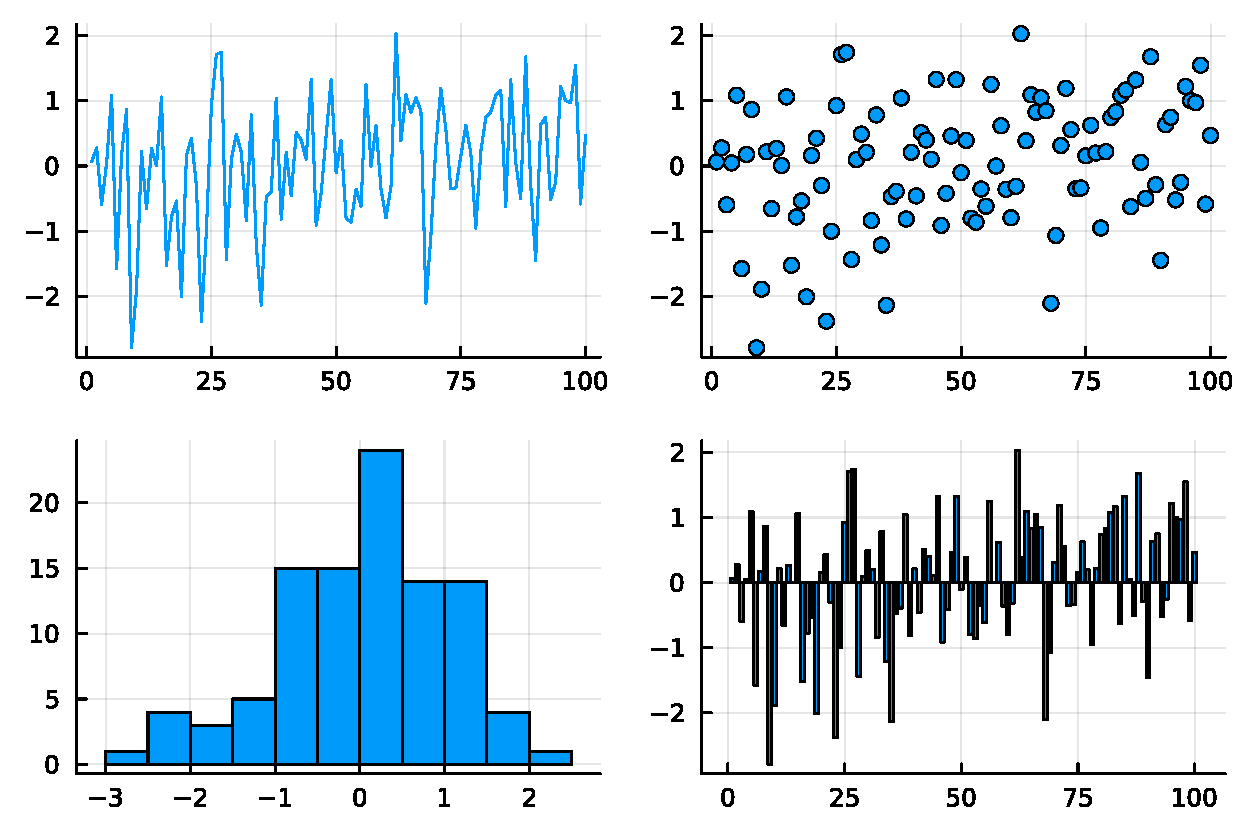
\includegraphics[width=.95\columnwidth]{pic.pdf}
\end{figure}

Ein weiteres Beispiel unter Verwendung von \lstinline|StatsPlots.jl|:
\begin{lstlisting}
#]add StatsPlots
using StatsPlots
using Distributions
using Plots
using Random
Random.seed!(42)
mu, sigma = 100, 15
x = mu .+ sigma * randn(10000)
histogram(x,
          title="Histogram of IQ: \\mu=100, \\sigma=15",
          label=nothing,
          xlabel="Smarts",
          ylabel="Probability",
          color="green",
          normalize=true)
plot!(Normal(mu, sigma),
      color="red",
      label=nothing,
      linestyle=:dash)
savefig("hist.pdf")
\end{lstlisting}

\begin{figure}[h]
\centering
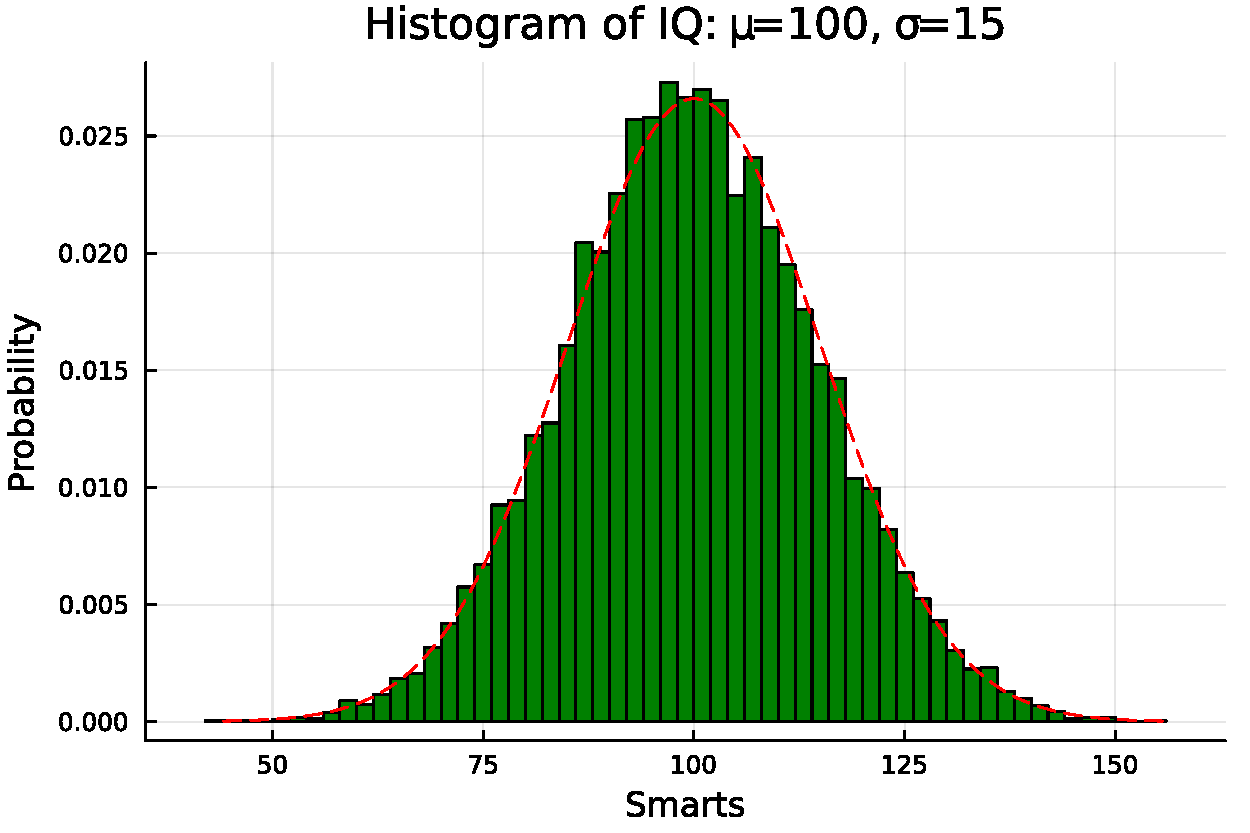
\includegraphics[width=.95\columnwidth]{hist.pdf}
\end{figure}

\section{Tabellen -- DataFrames}
\label{sec:dataFrame}

Neben \lstinline|DataFrames.jl| und \lstinline|CSV.jl| gibt es weitere Pakete
für den Umgang mit Tabellen.

Eine CSV--Datei einlesen.
\begin{lstlisting}
#]add DataFrames
#]add CSV
using DataFrames
using CSV
path = joinpath(dirname(pathof(DataFrames)),
        "../docs/src/assets/iris.csv")
df = CSV.read(path, DataFrame);
last(df, 3)   # Letzten 3 Datenzeilen
first(df, 3)  # Ersten 3 Datenzeilen
\end{lstlisting}

Ergibt die folgenden Ausgabe:
\begin{lstlisting}[basicstyle=\scriptsize]
3x5 DataFrame
 Row | SepalLength  SepalWidth  PetalLength  PetalWidth  Species
     | Float64      Float64     Float64      Float64     String
---------------------------------------------------------------------
   1 |         5.1         3.5          1.4         0.2  Iris-setosa
   2 |         4.9         3.0          1.4         0.2  Iris-setosa
   3 |         4.7         3.2          1.3         0.2  Iris-setosa
\end{lstlisting}

Wichtige Funktionen für das eben eingelesenen \lstinline|DataFrame| sind:

\begin{lstlisting}
DataFrame(a=1:10, b=rand(10))  # Erzeugt ein DataFrame
describe(df)                   # Information zu df
df.Species                     # Spalte Species
df[!, :Species]                #  Alternative
df[:, :Species]                # Macht eine Kopie
df[1, 5]                       # Wert in Zeile 1 Spalte 5
df[1:2, 3:4]                   # Zeilen 1:2, Spalten 3:4
Matrix(df[:, 1:4])             # Umwandlung in Matrix
names(df)                      # Spaltennahmen
nrow(df); ncol(df)             # Anzahl Zeilen; Spalten
sort(df, :SepalWidth)          # Sortiere nach SepalWidth
sort!(df, :SepalWidth)         #  In palce
filter(:SepalWidth => >(3), df)  # Neues df wo true
push!(df, (1, 2, 3, 4, "Some species")) # Zeile anhängen
df.key = axes(df, 1)           # Neue Spalte
 # Summe SepalLength je Species
combine(groupby(df, :Species), :SepalLength => sum)
 # Spalten 1:4 untereinander: wide -> long
df2 = stack(df, 1:4, [:key, :Species])
 # long -> wide
unstack(df2, [:key, :Species], :variable, :value)
\end{lstlisting}


%Autor: Georg Kindermann

\end{document}
